%=================================================================
\documentclass[article,accept,moreauthors,pdftex,10pt,a4paper]{Definitions/mdpi}
%\usepackage[lite]{mtpro2}
\usepackage{scalerel}
\firstpage{1} 
\makeatletter 
\setcounter{page}{\@firstpage} 

\Title{Laser Calibration System - Analysis of the Local Monitors}

% Authors, for the paper (add full first names)
\Author{Nandita Raha, $~INFN ~Pisa$}


\abstract{
%The Muon g-2 experiment at Fermilab will measure the 
%anomalous magnetic moment of the muon to a precision of 140 parts per billion 
%compared to the previous measurement at 540 parts per million of E821 
%by increasing statistics and using upgraded apparatus. 
%One of the essential requirement is an improved highly sophisticated 
%Laser calibration system that uses a novel technique to calibrate the calorimeters 
%used to detect the decay positrons in a penning trap. The calibration system distributes 
%laser light to calibrate all channels of all the calorimeters. The stability of 
%the laser source itself is checked using  source monitors and the stability of the optical 
%distribution chain and the source monitor is performed using the local monitors. 
This document analyzes the local monitor data from a dataset of the first data--taking run 
(an accumulation of 60 hours of runs) and also performs some simulations 
to check the local monitor performance. It also tests if any long-term 
corrections related to temperature fluctuations, 
humidity etc. are essential or not for the local monitors at the 
desired level of precision of the experiment.}
\begin{document}
%\setcounter{section}%{} %% Remove this when starting to work on the template.

\section{A reminder of the laser calibration system}
The schematic of the calibration system is shown in Figure \ref{fig1}. 
We use six laser heads (LDH-P-C-405 M by PicoQuant) that provide up to 
1 nJ of pulses 700 ps wide at a wavelength of 405 nm to calibrate all the 
calorimeters \cite{anas}. The light from each laser is divided in a ratio of 
70:30 by a beam splitter. The 70\% light is further divided into four equal
parts and transported to the four calorimeters in
the ring using 25 m-long quartz optical fibers via a diffuser (to convert the 
Gaussian distribution of light intensity into a more uniform and flat distribution) and a fiber bundle. 
This delivers light to each of the 54 $PbF_2$ crystals with the fiber bundle attached to a 
Delrin panel embedded with optical prisms located in front of the calorimeter. 
A Source Monitor (SM) is used to measure pulse-by-pulse
the intensity of the remaining 30\% of the laser light \cite{c2}. 
\begin{figure}[H]
\centering
%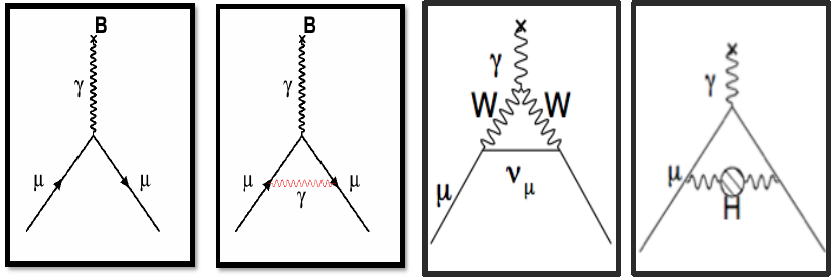
\includegraphics[width=2 cm]{a_mu_corrections.png}
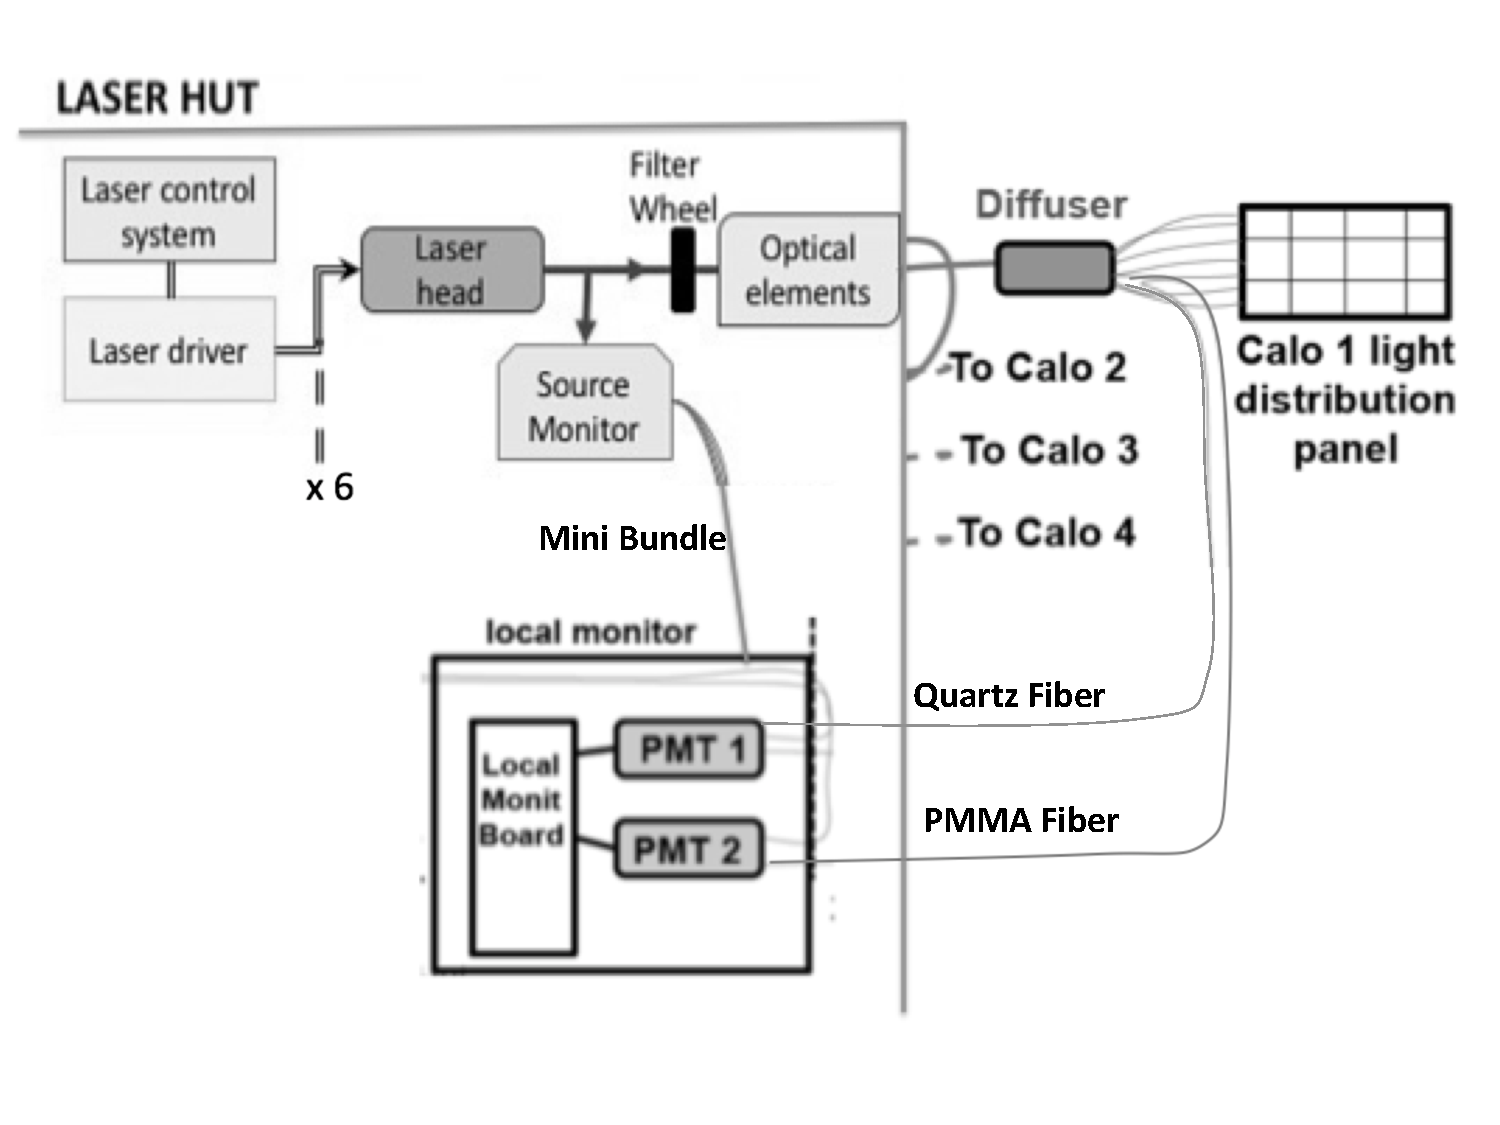
\includegraphics[width=9 cm]{laser_sys.pdf}
%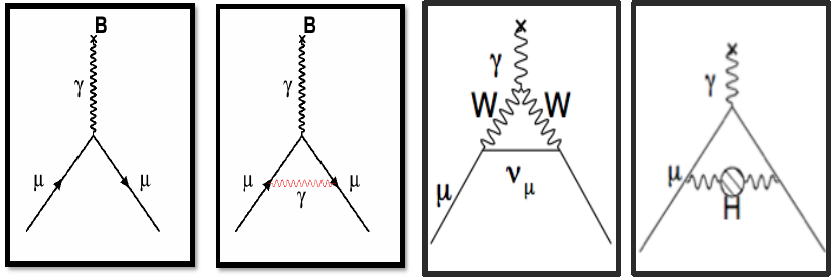
\includegraphics{a_mu_corrections.pdf}
\caption{\label{fig1}A schematic showing the laser calibration system. }
\end{figure} 
The optical stability of this entire system is checked 
using a Local Monitor (LM). A mini-bundle fiber transmits 
light from the SM to the LM. Each LM consists of a PMT 
which collects this light from the SM and is used as a reference signal. 
This has an amplitude of A1 (amplitude is defined as the pedestal subtracted 
peak adc value of the waveform). The light from the optical elements, 
the diffuser, the 25 m quartz fiber (that transmits light to the calorimeter) is
transmitted back to this PMT using by a quartz fiber. This has an amplitude of A2.
However, certain calorimeters, namely 11, 12, 13, 18 and 20 used an additional 
old PMT. For these calorimeters, the light from the optical system to the PMT was 
transmitted using a PMMA fiber. This was done to investigate the properties of the 
fiber used for transmission of light and also 
for a comparison between the old and the new PMTs.
The stability of this distribution system is quantified by comparing the ratio of light
from the two sources i.e. A2:A1. 

 
%The optical system, 25 m quartz fiber that transmit 
%light to calorimeters (forward fiber) and the the light transmitted via 
%the PMMA is from the calorimeters to the LM (return fiber) 
%are all included in A2.  

\section{A study using old and new PMTs of the LM}
The major goal is to check if the fluctuations in the LMs gain due to various 
external factors like temperature, humidity etc. will have an effect on 
the SiPMs gain calibration. Thus we begin by studying the stability of the LM for a 
long period of time. We considered a 60--hour data set of run 1 for consistency checks.  
Run numbers from 15920 to 15990 dated 22/4 (1:09 pm) to 25/4 (2:20 am) 
where precisely considered for our study.  
\begin{figure}[H]
\centering
%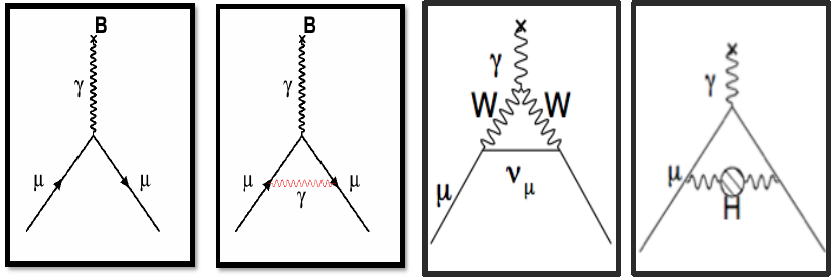
\includegraphics[width=2 cm]{a_mu_corrections.png}
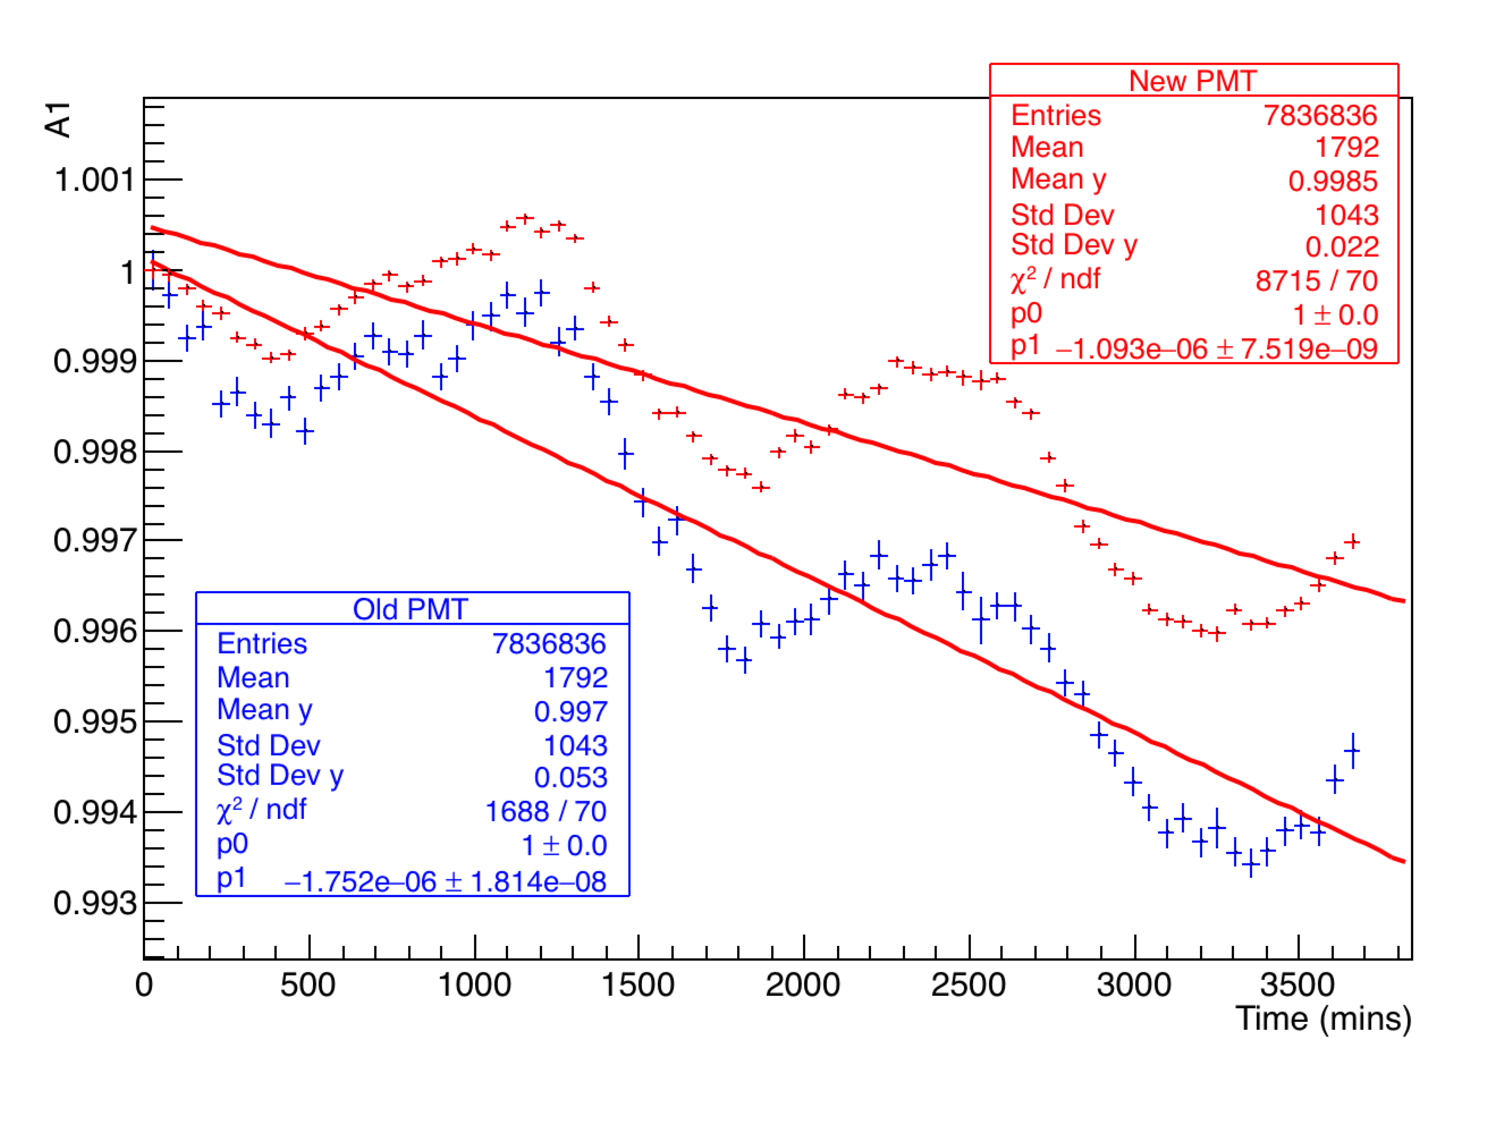
\includegraphics[width=5 cm]{calo20_a1_60hr.pdf}
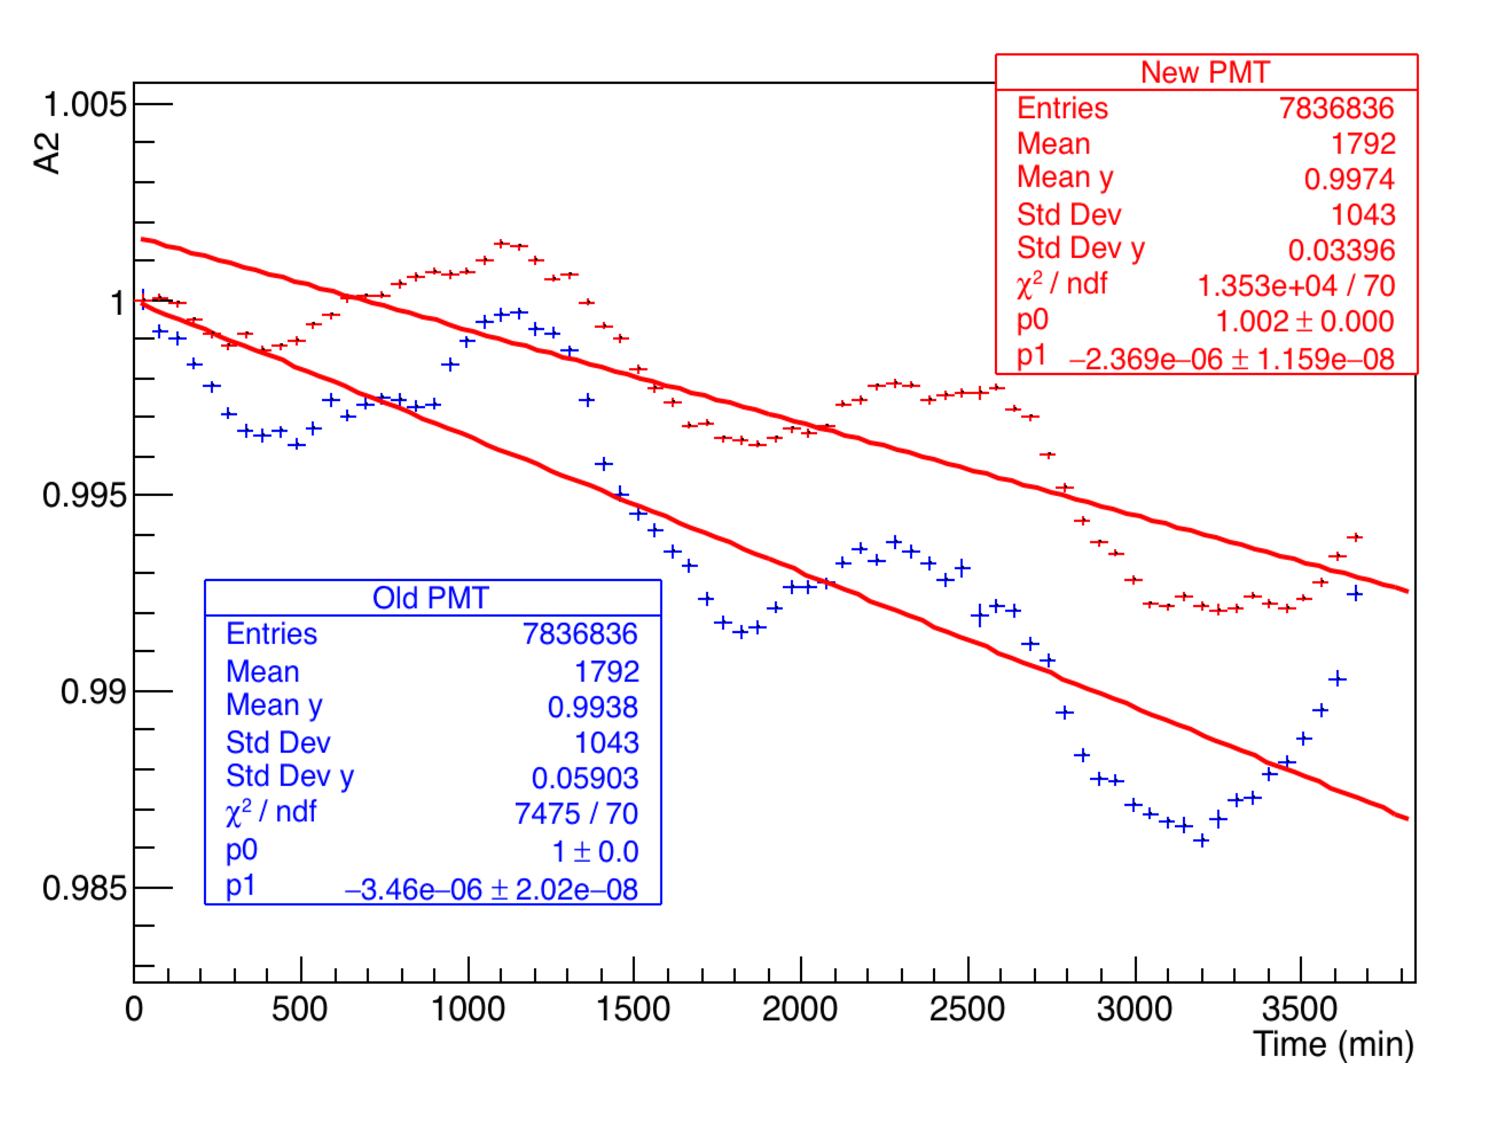
\includegraphics[width=5 cm]{calo20_a2_60hr.pdf}
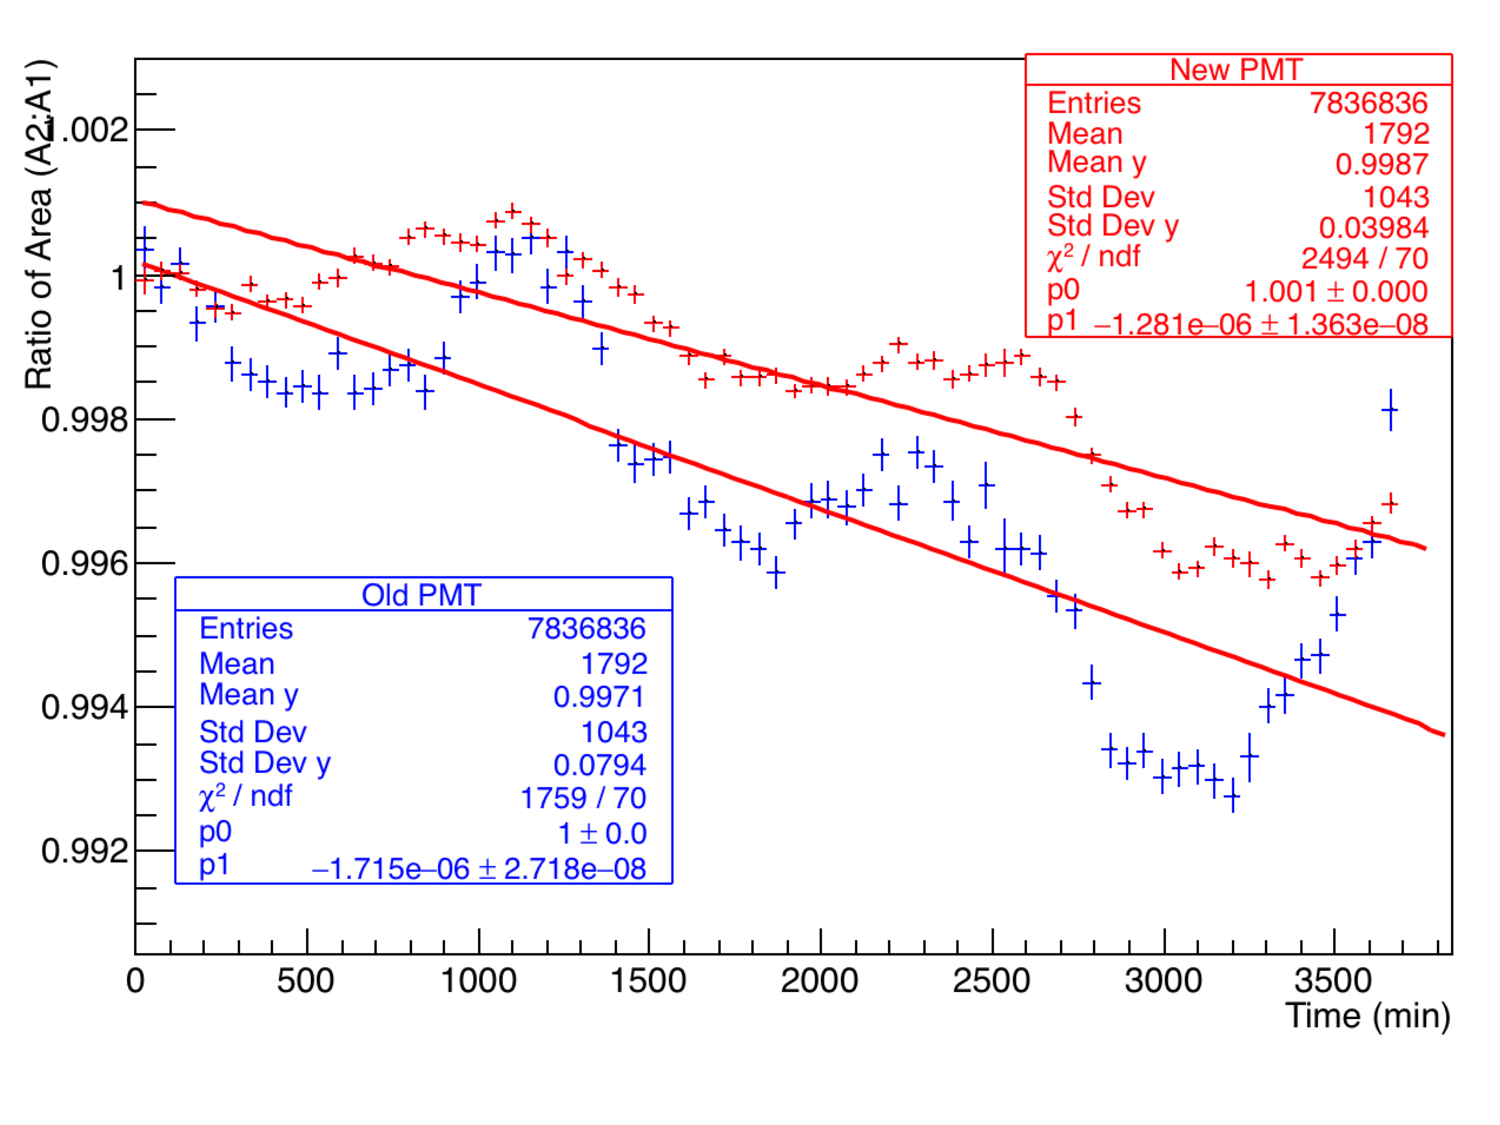
\includegraphics[width=5 cm]{calo20_a2_a1_60hr.pdf}
%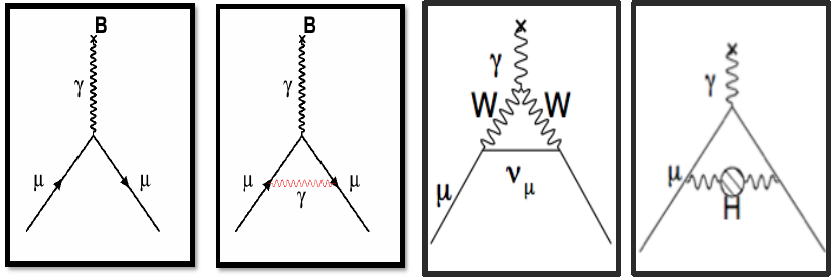
\includegraphics{a_mu_corrections.pdf}
\caption{\label{fig2}Comparing old (blue) and new (red) PMTs of the 60--hour dataset from run1. The left plot 
denotes variation of A1 with time. The middle plot denotes the same for A2 and the right plot denotes 
the fluctuation of A2:A1 with time.}
\end{figure}  

%Almost all LMs use a single PMT (which are new PMTs) expect a few calorimeters namely 11, 12 ,13, 18 and 20 
%which use two PMTs, a new PMT (with a quartz return fiber) and an old one (with a PMMA return fiber). 
%This was done to investigate the properties of the fiber used for transmission of light and also 
%for a comparison between the old and the new PMTs. 
Figure \ref{fig2} compares the fluctuations of 
the old (in blue) and the new (in red) PMT channels respectively of the LM connected to calorimeter 20. 
The PMT of the LM is connected to SM with a very short fiber and so A1 practically denotes the gain 
of the PMT. On the hand, A2 includes various transmission fibers, diffuser and other optical elements 
and thus has a much larger drop (almost twice as that of A1, as is evident in 
the data - refer to figure \ref{fig2}). Since A2:A1 denotes the stability or fluctuation of the entire optical 
system along with the monitoring system, its drop (or fluctuation) is comparable or dominated by A2 as is evident 
in the right plot of figure \ref{fig2}. 
\begin{figure}[H]
\centering
%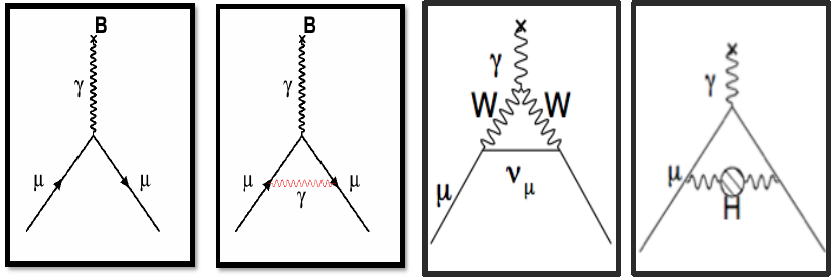
\includegraphics[width=2 cm]{a_mu_corrections.png}
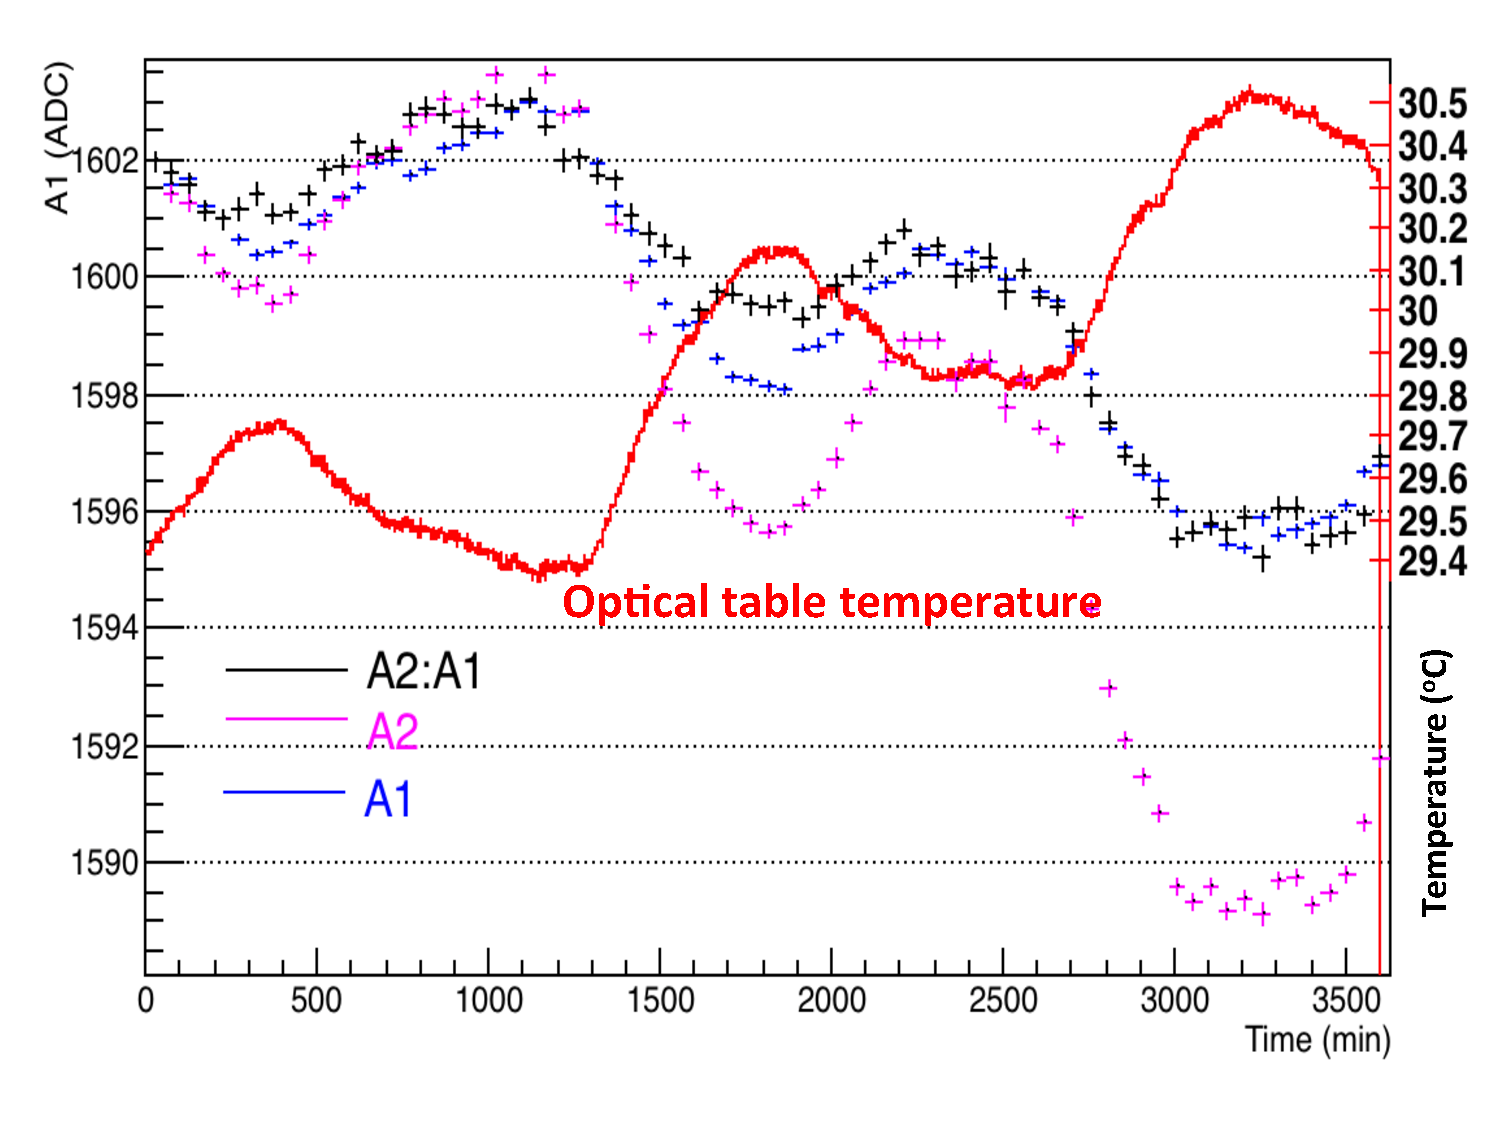
\includegraphics[width=9 cm]{temp_amp_60hr.pdf}
%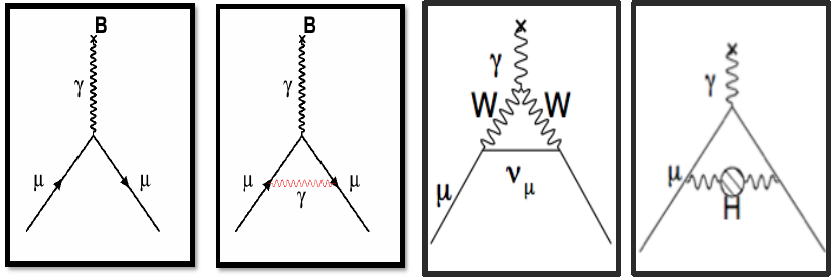
\includegraphics{a_mu_corrections.pdf}
\caption{\label{fig3}Effect of temperature on the LMs.}
\end{figure} 
Note that we use linear fits in these plots which do not correctly 
represent the data but is reasonable to get a rough estimate of the drop in gain per minute for the 60 hours runtime. 
These plots also show that the old PMTs in all cases have a larger drop in gain (about 1.5 times more than the 
new ones). This could be due to aging or improper configuration of voltage settings or light intensities. 
The voltage settings of only the new PMTs were configured according to the light intensity from the filter wheel settings. 

%%%%%%%%%%%%%%%%%%%%%%%%%%%%%%%%%%%%%%%%%%
\subsection{Effect of environmental factors on the performance of LMs}
In the longer run (datasets of more than one day or so), it is important to check the effect of 
various environmental factors on the performance of the LMs. This mainly includes temperature and 
other minor factors like humidity, air pressure etc. The temperature with these minor corrections applied 
was read from the database for this dataset and exhibits a diurnal effect (peaks during the day and is low at night) 
as shown by the red plot in figure \ref{fig3}. 

The temperature range for this 60--hour dataset is about 1.1 $^o$C. The blue, pink and black plots show the variation of 
A1, A2 and A2:A1 respectively with time. A2 and A2:A1 are all normalized to the initial 
value of A1 and all the three plots are overlaid on the same plot to compare. 
This clearly shows a negative correlation of the gains with temperature (as the 
temperature increases these amplitudes decrease). To quantify this drop with temperature, we found the correlation of 
temperature with each of A1, A2 and A2:A1 as shown in figure \ref{fig4} for the same channel.

\begin{figure}[H]
\centering
%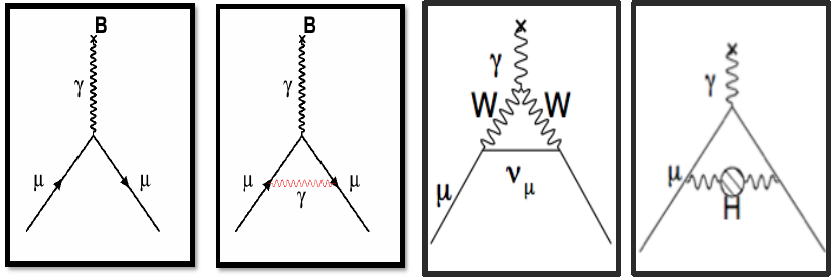
\includegraphics[width=2 cm]{a_mu_corrections.png}
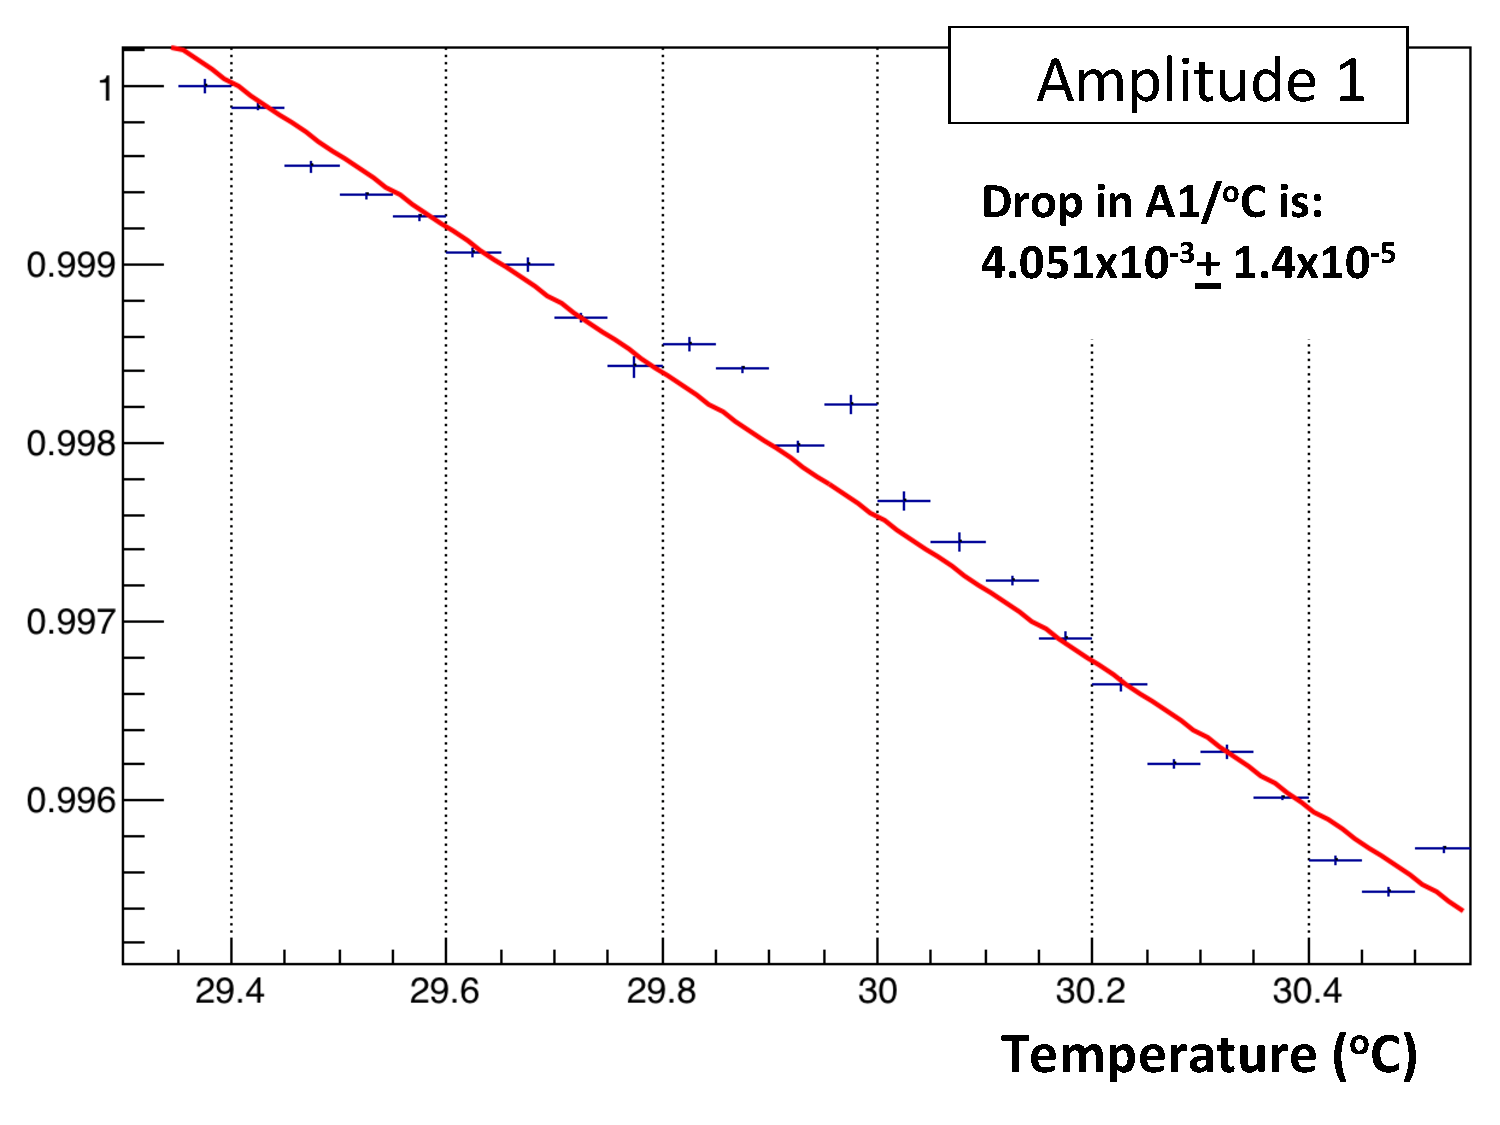
\includegraphics[width=5 cm]{amp1_temp_60hr.pdf}
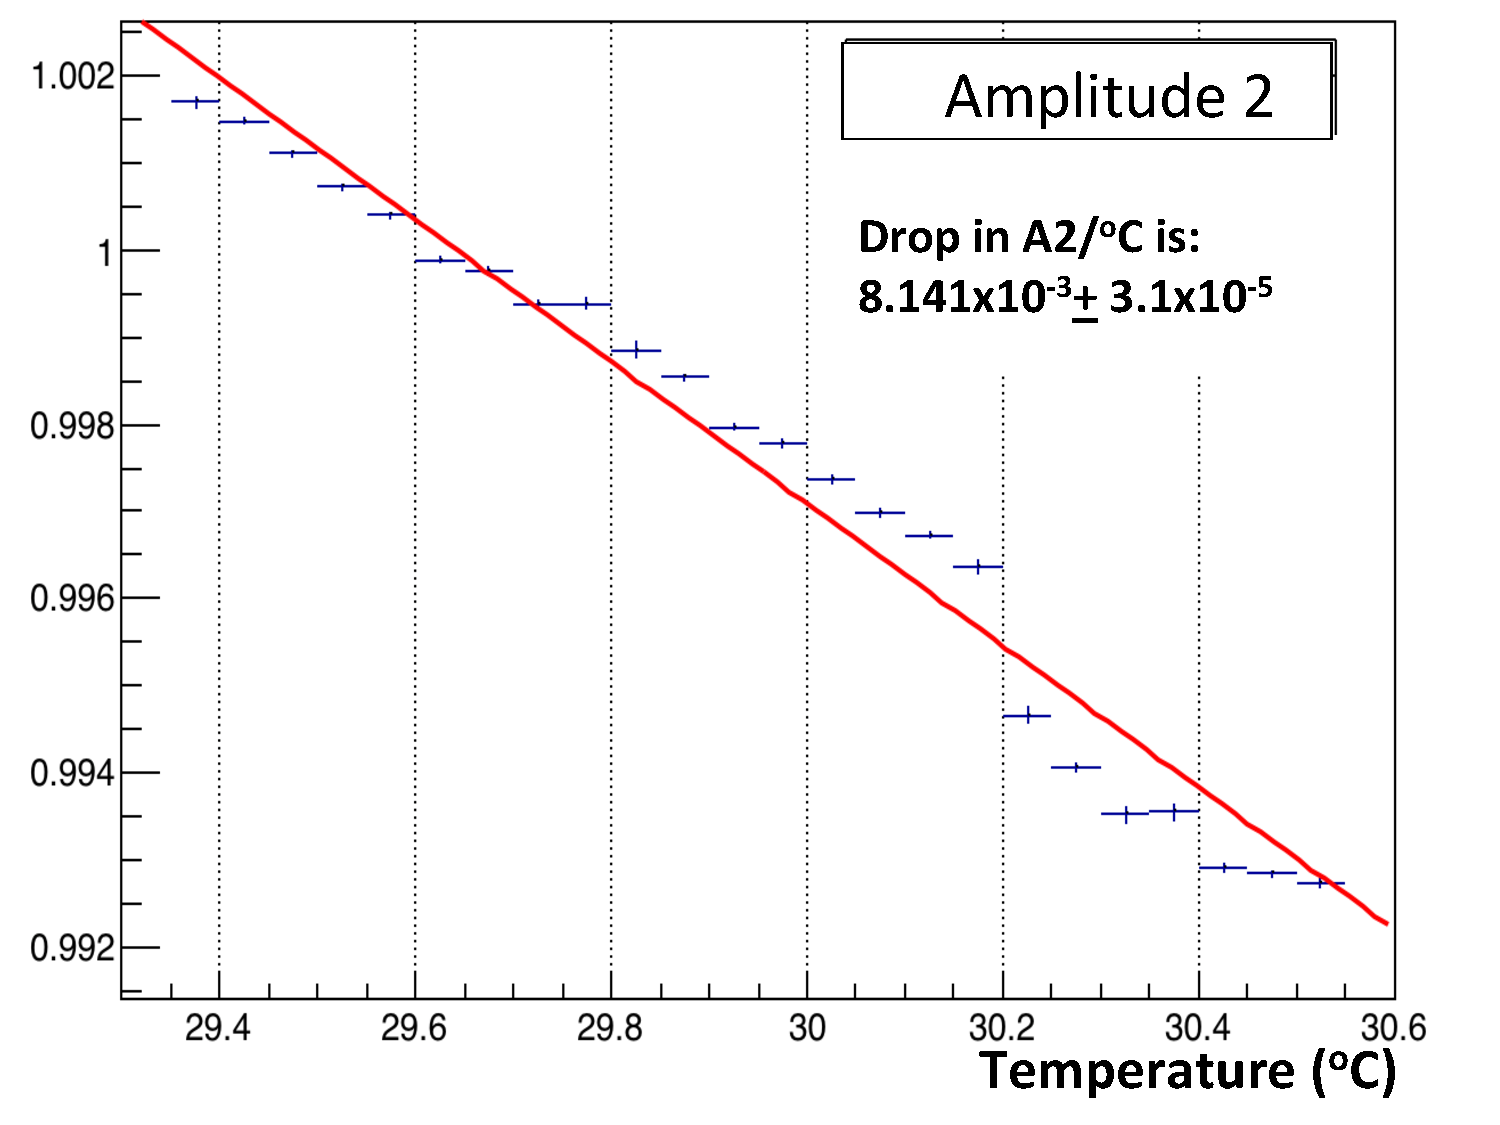
\includegraphics[width=5 cm]{amp2_temp_60hr.pdf}
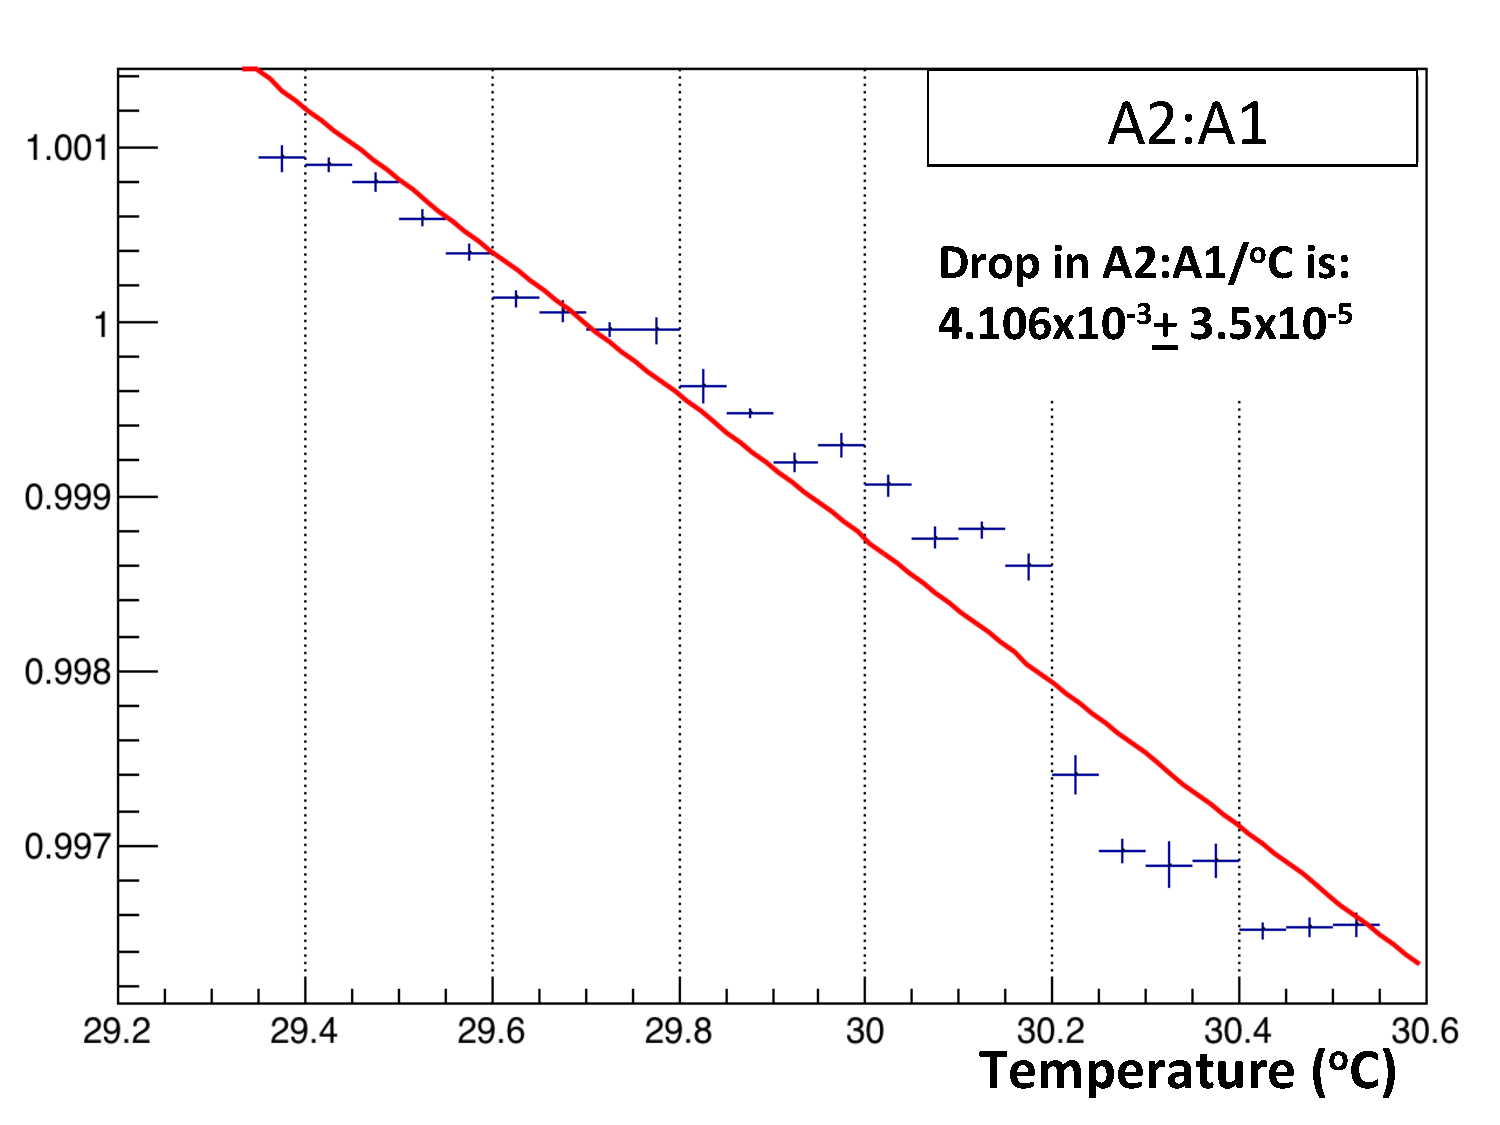
\includegraphics[width=5 cm]{a2_a1_temp_60hr.pdf}
%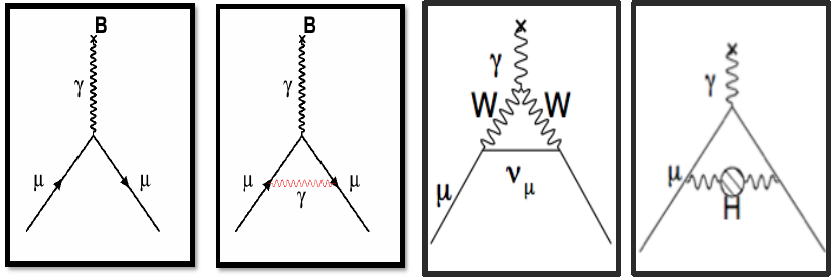
\includegraphics{a_mu_corrections.pdf}
\caption{\label{fig4}Variation of amplitude with temperature for a PMT channel of the 60--hour dataset. }
\end{figure}  
To study the behaviour of the gain drops with temperature for all channels of the LM 
(from all 24 calorimeters), we find the correlation of A1, A2 and A2:A1 with temperature for each 
channel (a plot like figure \ref{fig4}) and perform a linear fit. The slope of this fit with its error 
estimates the drop in these quantities with temperature. The absolute value of these drops are plotted 
in the graphs of figure \ref{fig5} for each channel.
\begin{figure}[H]
\centering
%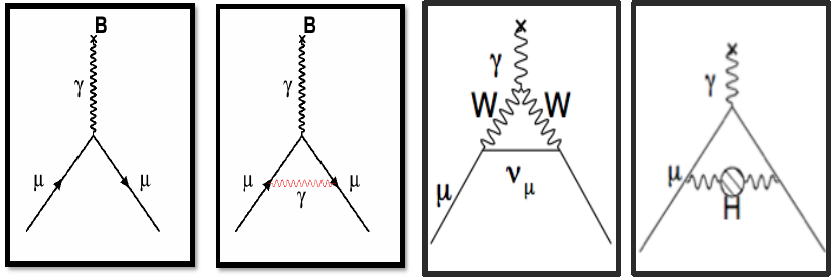
\includegraphics[width=2 cm]{a_mu_corrections.png}
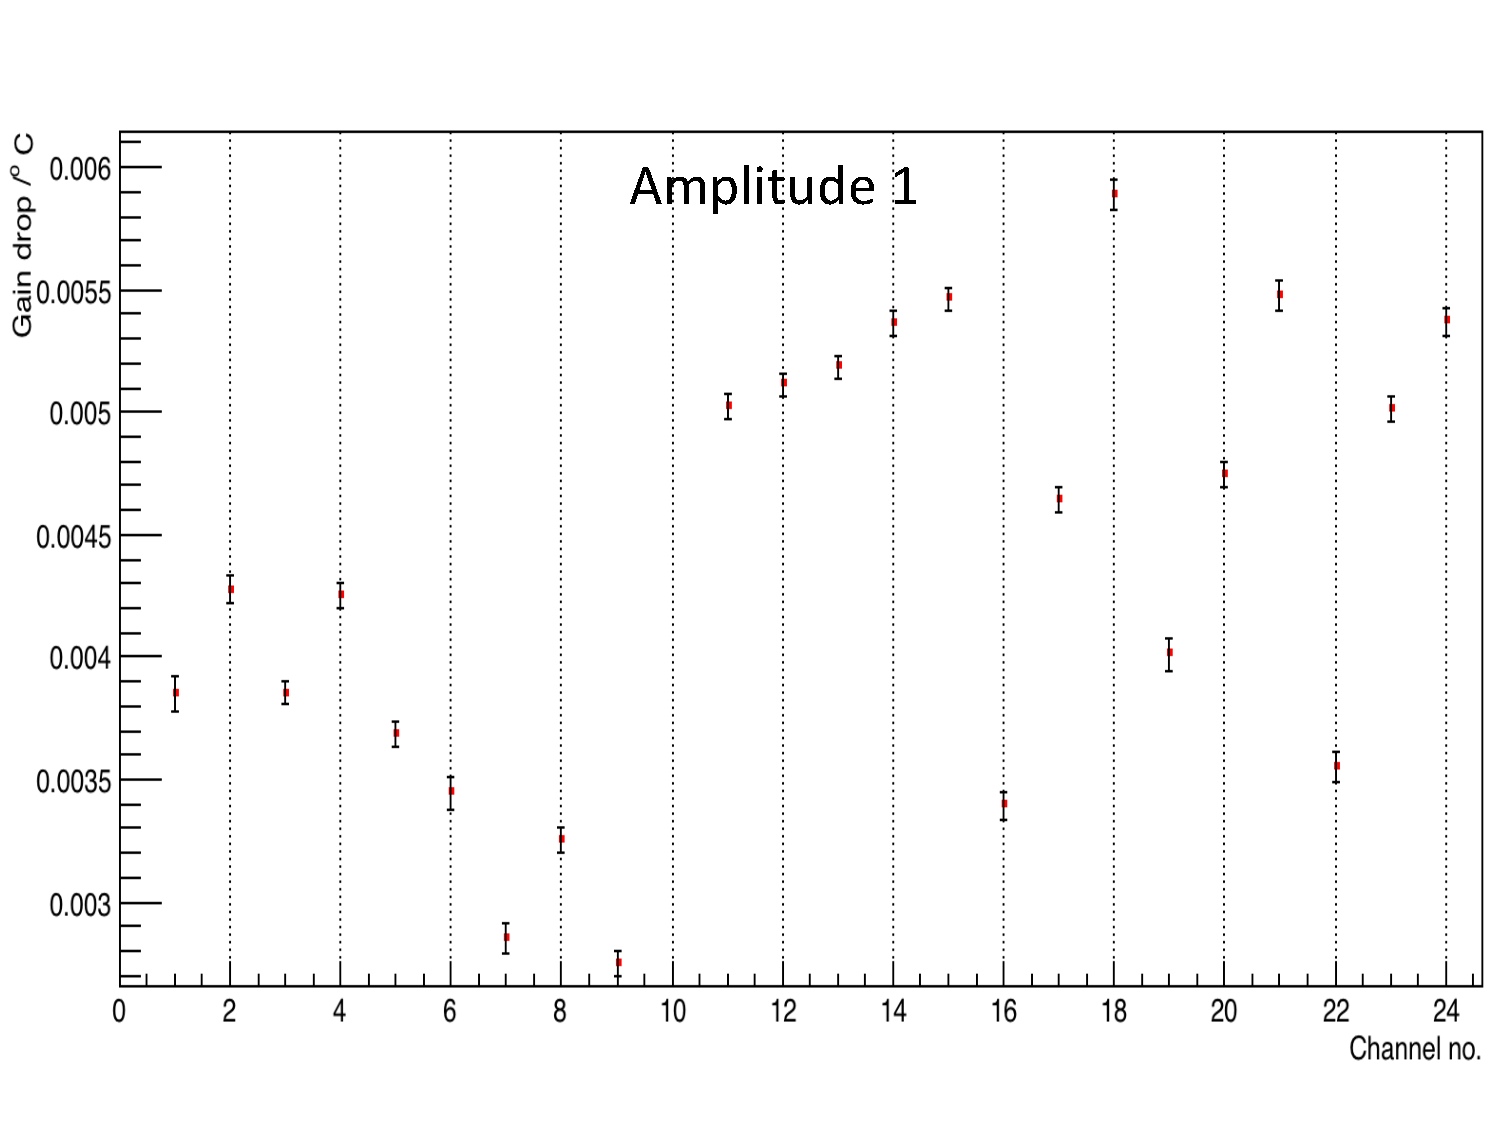
\includegraphics[width=5 cm]{All_amp1_temp_60hr.pdf}
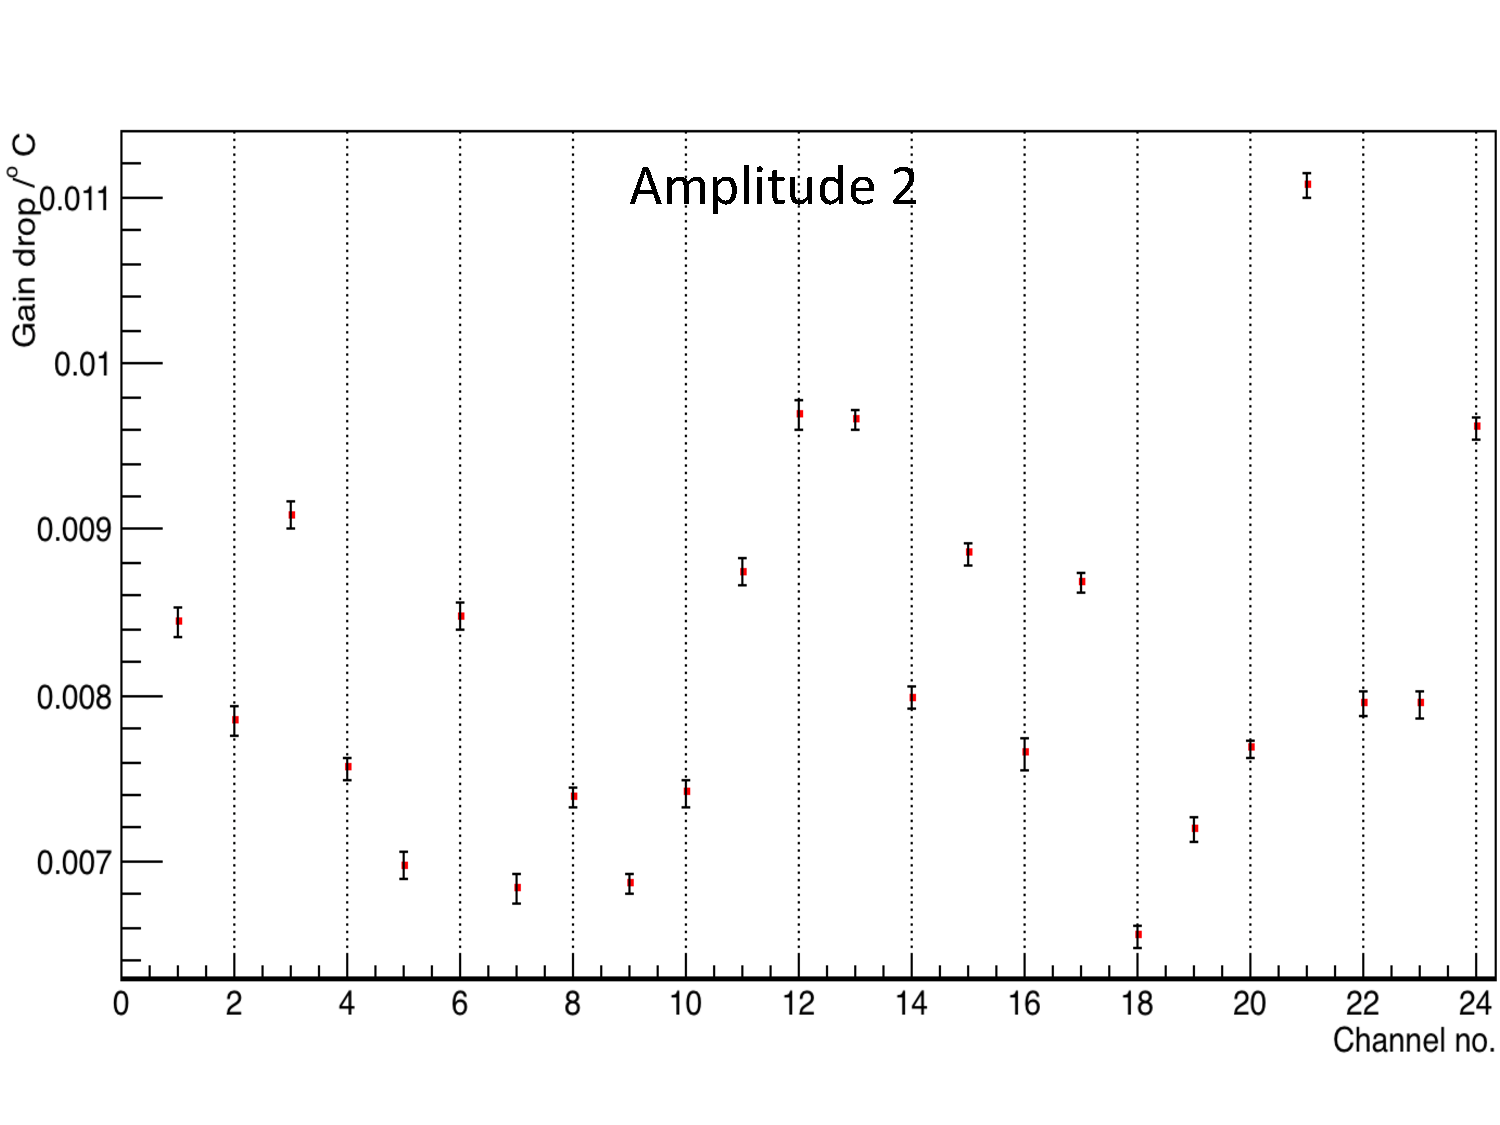
\includegraphics[width=5 cm]{All_amp2_temp_60hr.pdf}
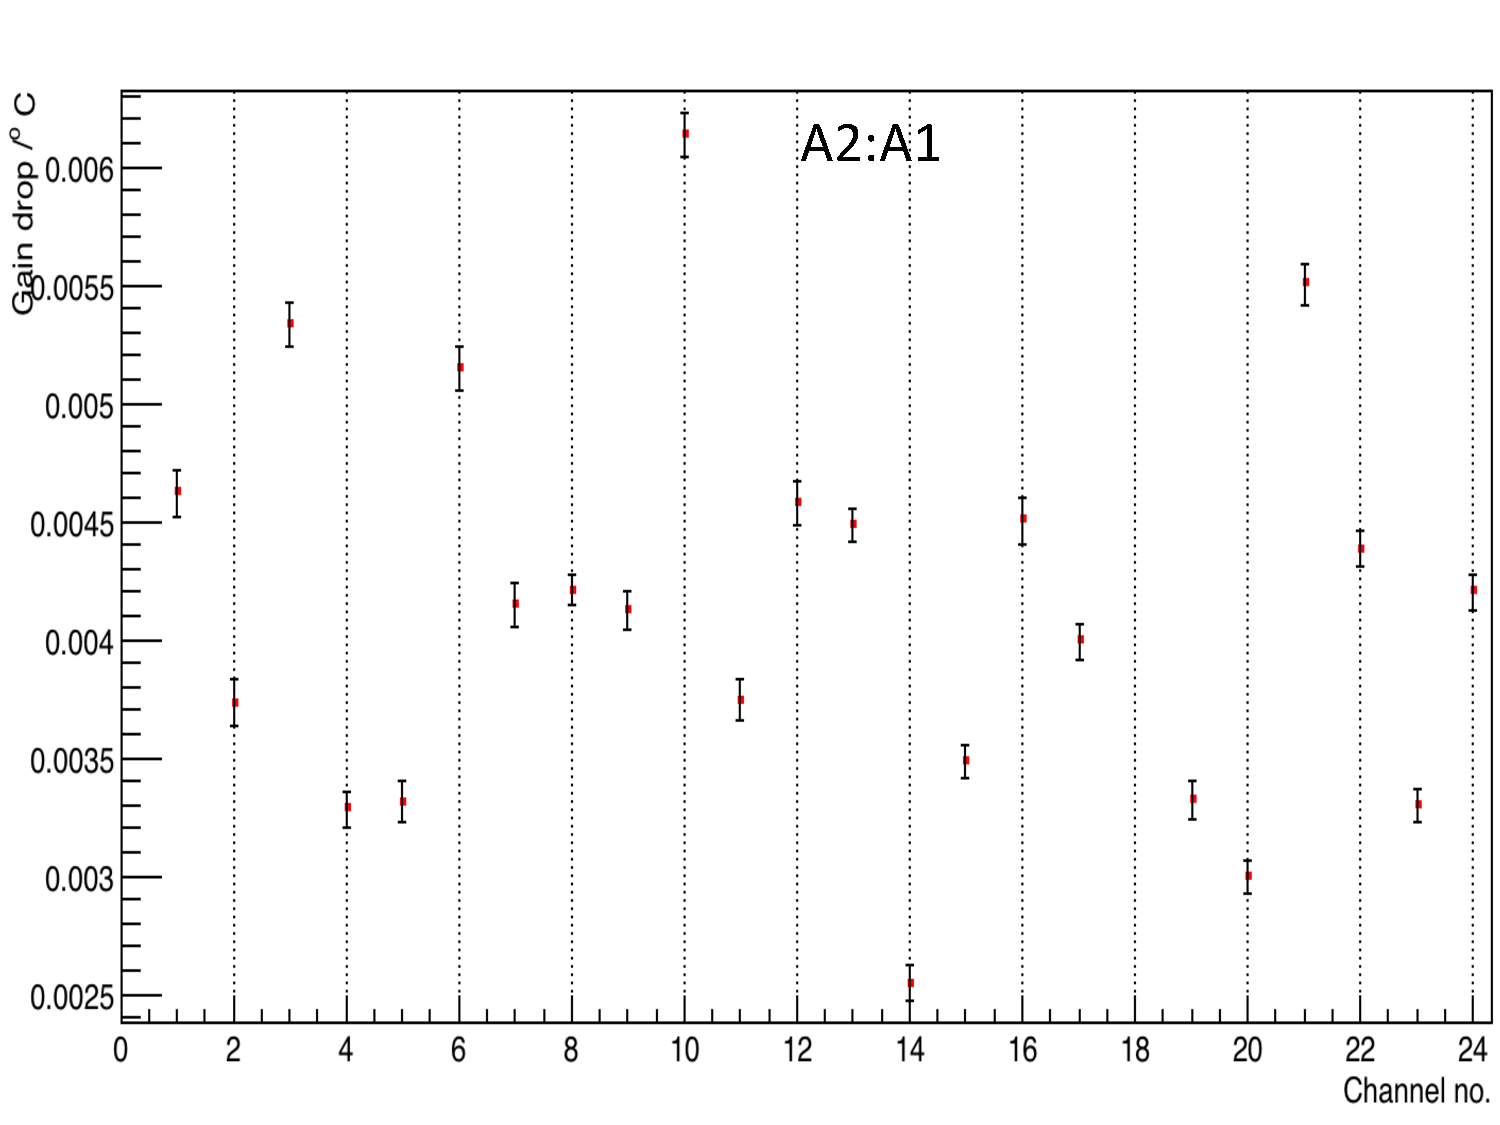
\includegraphics[width=5 cm]{All_a2_a1_temp_60hr.pdf}
%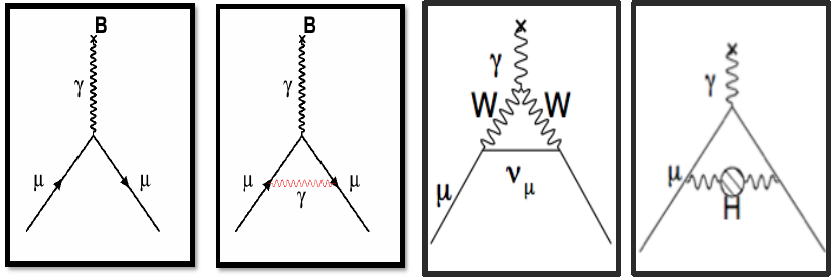
\includegraphics{a_mu_corrections.pdf}
\caption{\label{fig5}Drop of A1(left) A2(middle) and A2:A1(right) of all channels with temperature for the 60 hour dataset. }
\end{figure} 
\subsection{Effect of the connecting fiber on the performance of LMs}
Irrespective of the temperature, the PMMAs have a much greater loss in gain 
compared to the silica fibers. To investigate this we recently took a special 
24--hour long run. One of the channels was connected to the LM with 
PMMA while another was connected using a silica fiber from the 
calorimeters. Thus, A2 would show the effect of the type of 
fiber used, whereas A1 should be comparable for both channels. 
Both channels do show a negative correlation with temperature as 
expected but the drop in PMMA (left plot of figure \ref{fig7}) is more than 
3 times larger compared to the drop in silica fiber (right plot of figure \ref{fig7}).

%%%%%%%%%%%%%%%%%%%%%%%%%%%%%%%%%%%%%%%%%%
\begin{figure}[H]
\centering
%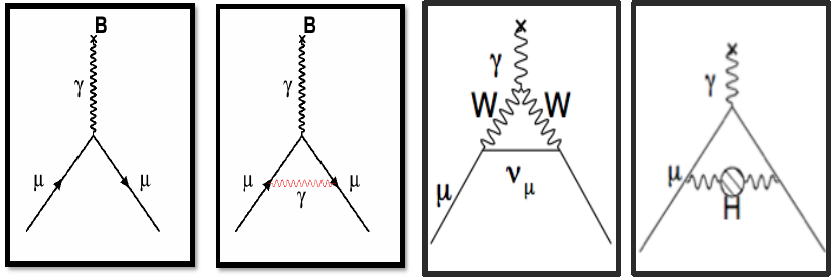
\includegraphics[width=2 cm]{a_mu_corrections.png}
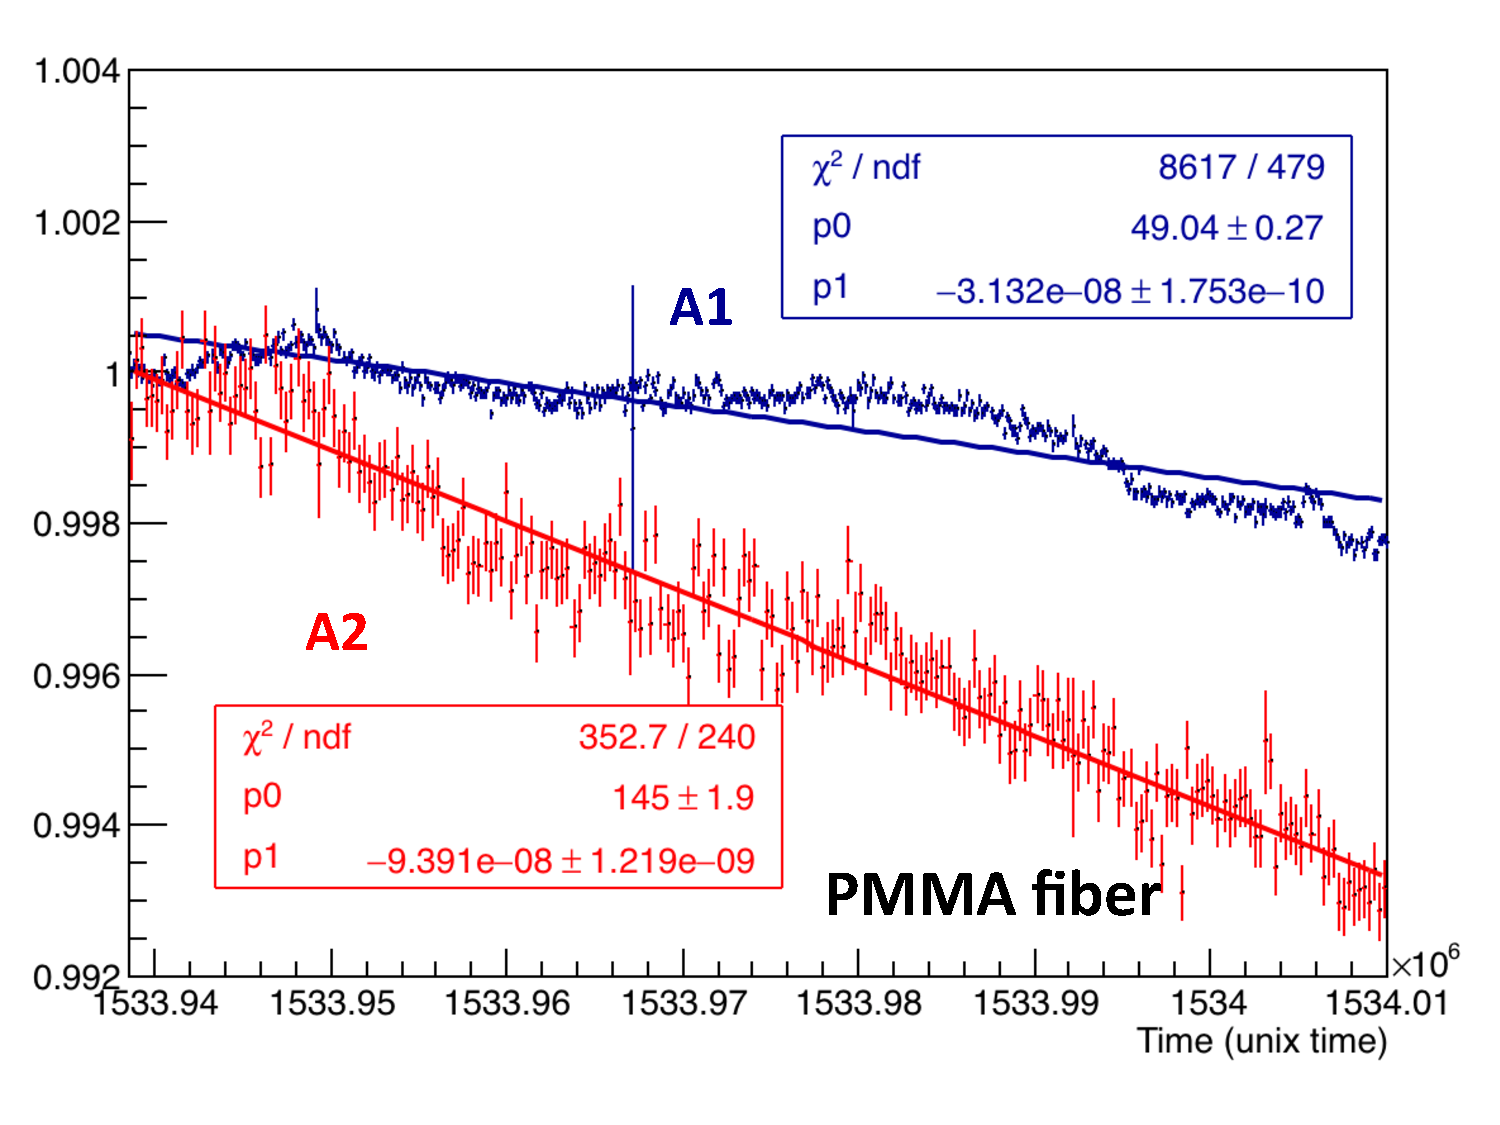
\includegraphics[width=7 cm]{PMMA.pdf}
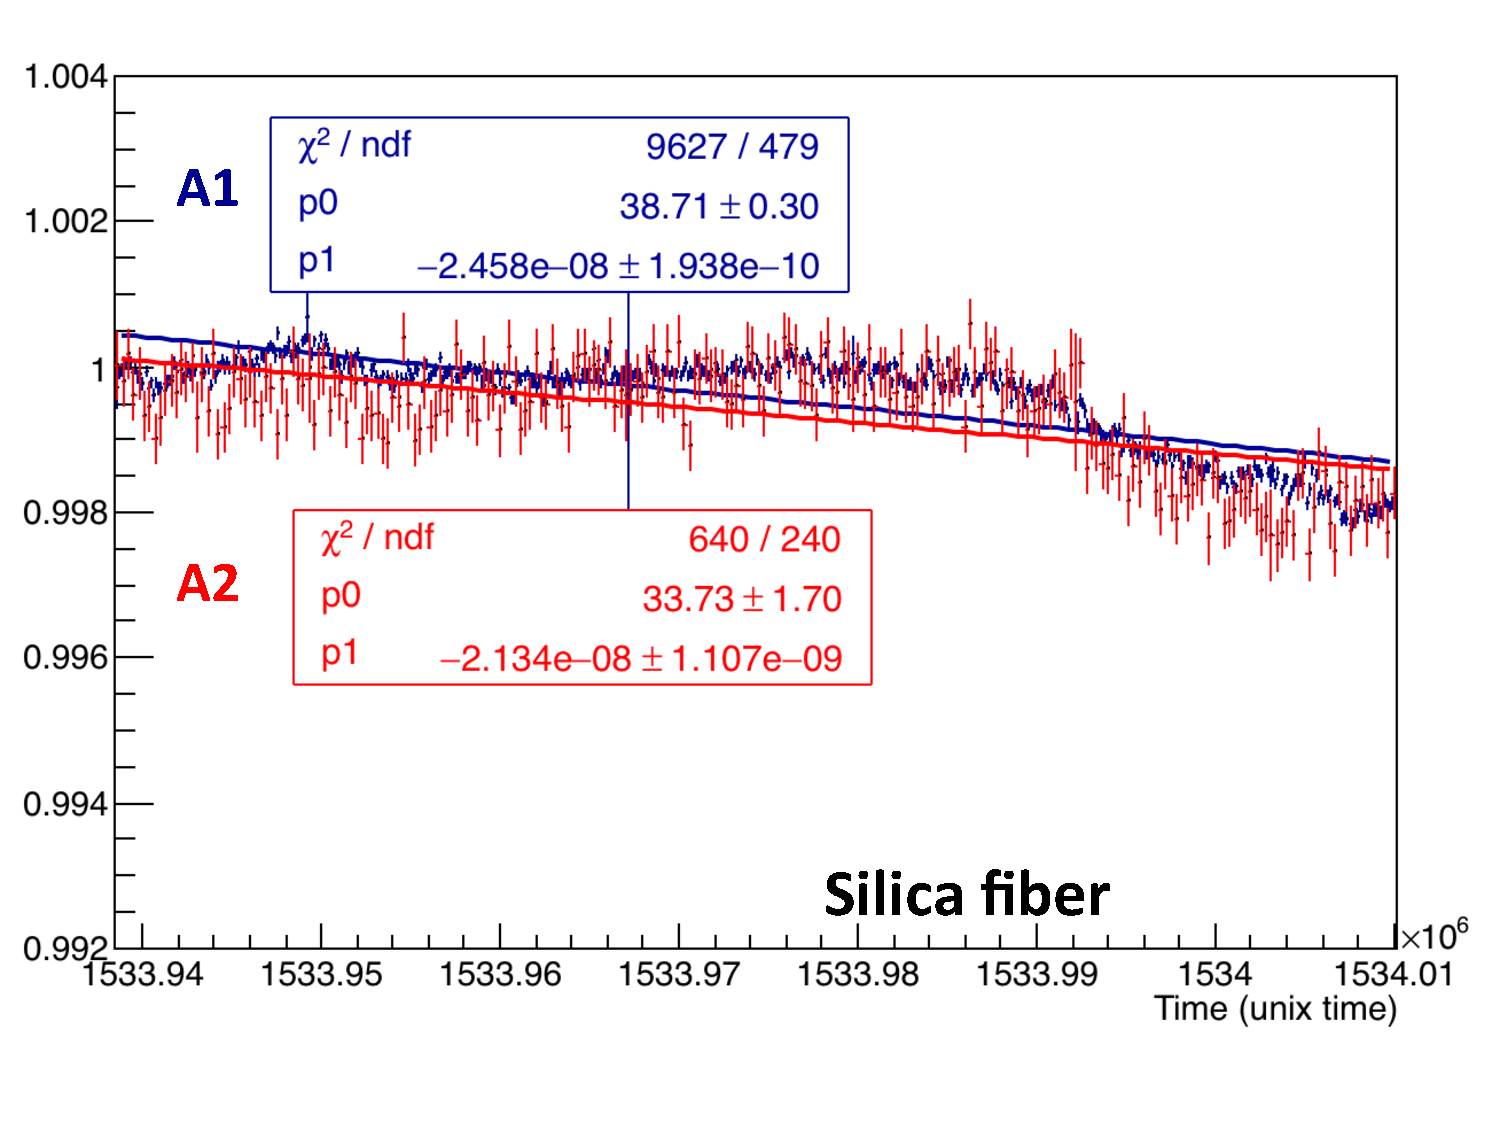
\includegraphics[width=7 cm]{silica.pdf}
\caption{\label{fig6}Difference between a silica fiber (right) and PMMA (left) one. }
\end{figure}  

%%%%%%%%%%%%%%%%%%%%%%%%%%%%%%%%%%%%%%%%%%
\section{Effect of LM fluctuations on SiPM gain function - a simulation}
To investigate the effect of these LM gain fluctuations on the SiPM gain 
functions used by the calorimeters we simulated this gain within a fill. 
A fill is a 700 $\mu s$ muon beam time. The beam is structured as 
two bunches of eight such fills constituting a cycle (i.e. 16 fills in a cycle) \cite{TDR}. 
The red plot in the right side of figure \ref{fig7} represents the standard gain function 
within a fill given by,
\begin{equation}
\begin{aligned}
&G(t) = 0.992(1-0.04e^{\frac{-t}{30}})
\end{aligned}
\end{equation}  
The asterisk (*) represent the points simulated by laser pulses. 
Three laser pulses are shot at 30 $\mu s$, 200 $\mu s$ and 400 $\mu s$ 
within a fill. After every 9 fills we move the laser pulse by an offset of 
2.5 $\mu s$ to obtain all simulated points within a fill as shown on the 
right side of figure \ref{fig7}. The data of the LM (A1) is plotted and 
fitted with a sinusoidal decreasing function (left side of figure \ref{fig7}). 
This resembles the diurnal temperature effect (with an anticorrelation) and fits the data better than 
a straight line. So we took this function for out-of-fill pulses for both the source 
and local monitors and took an average of the ratio of SiPM gain function (Q) with 
SM gain (S0) and LM gain (L0) over a sub run (i.e. about five cycles), given by,
\begin{equation}	
                       \begin{aligned}	
                       &\Bigg \langle \frac {(\frac{Q}{S0\times L0})_{i}}{\langle {\frac{Q}{S0\times L0}}\rangle}_{OOF}\Bigg \rangle	
                       \end{aligned}
\end{equation}  
  

\begin{figure}[H]
\centering
%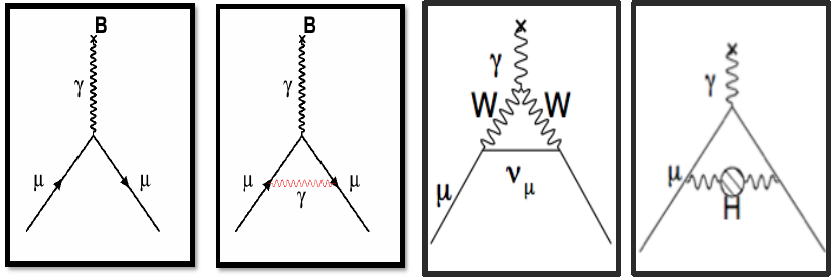
\includegraphics[width=2 cm]{a_mu_corrections.png}
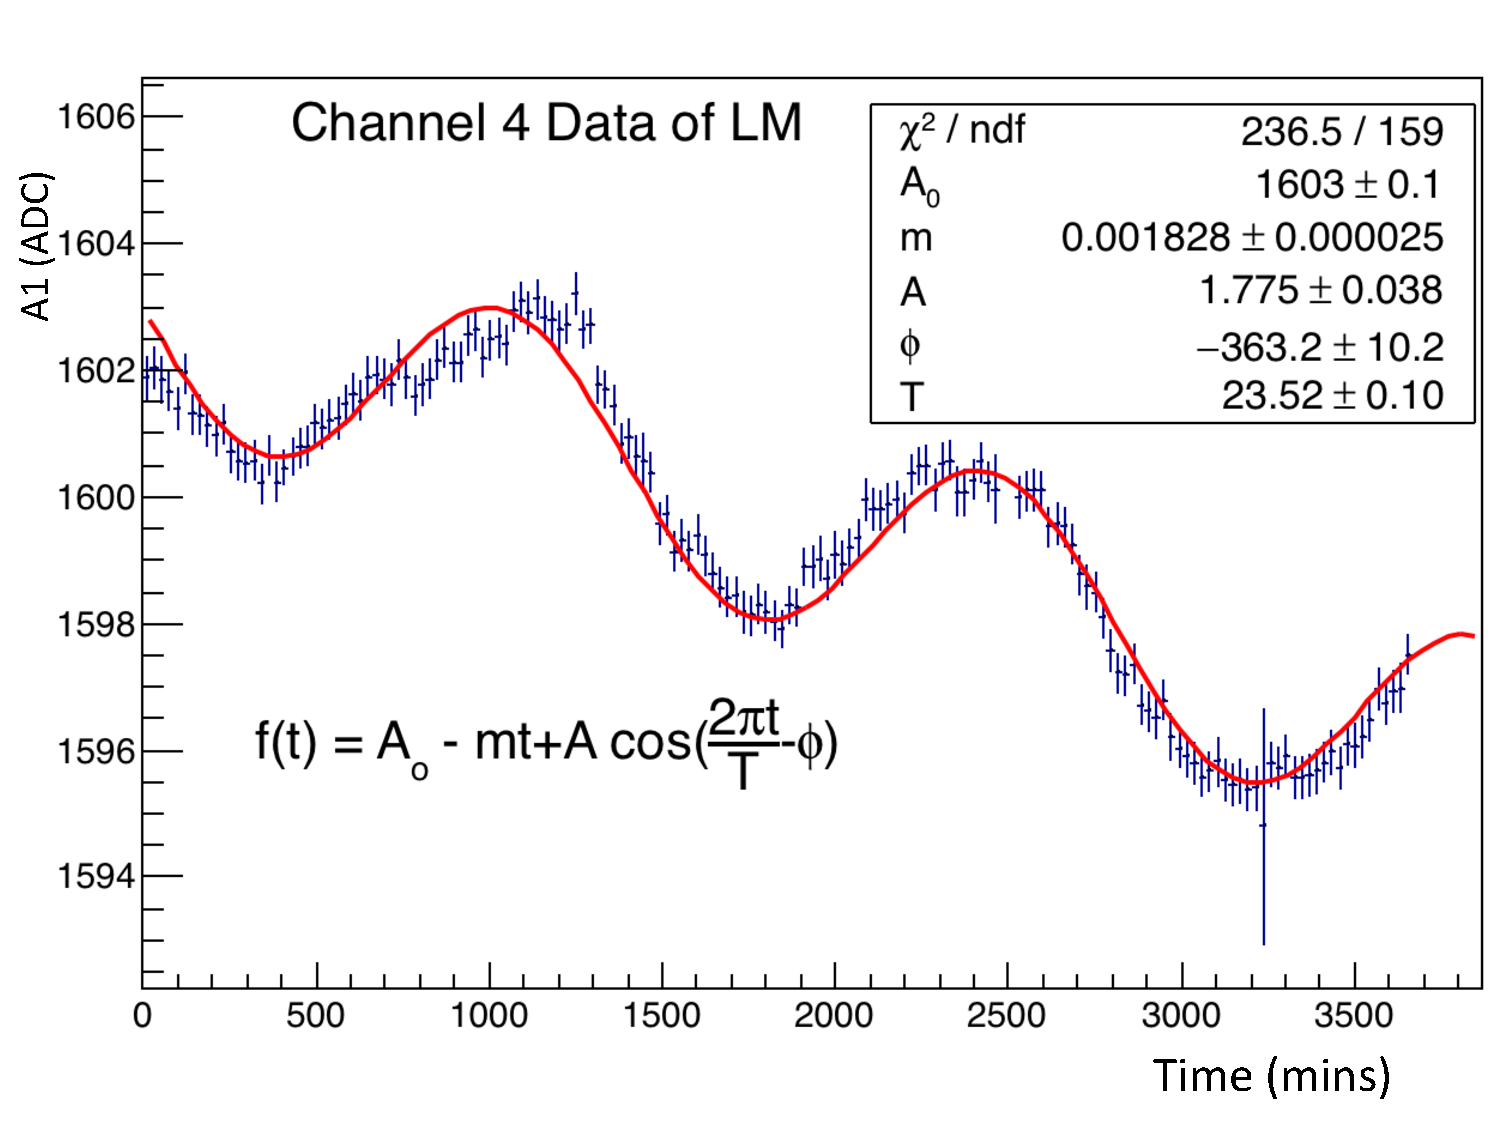
\includegraphics[width=7 cm]{LM_gain.pdf}
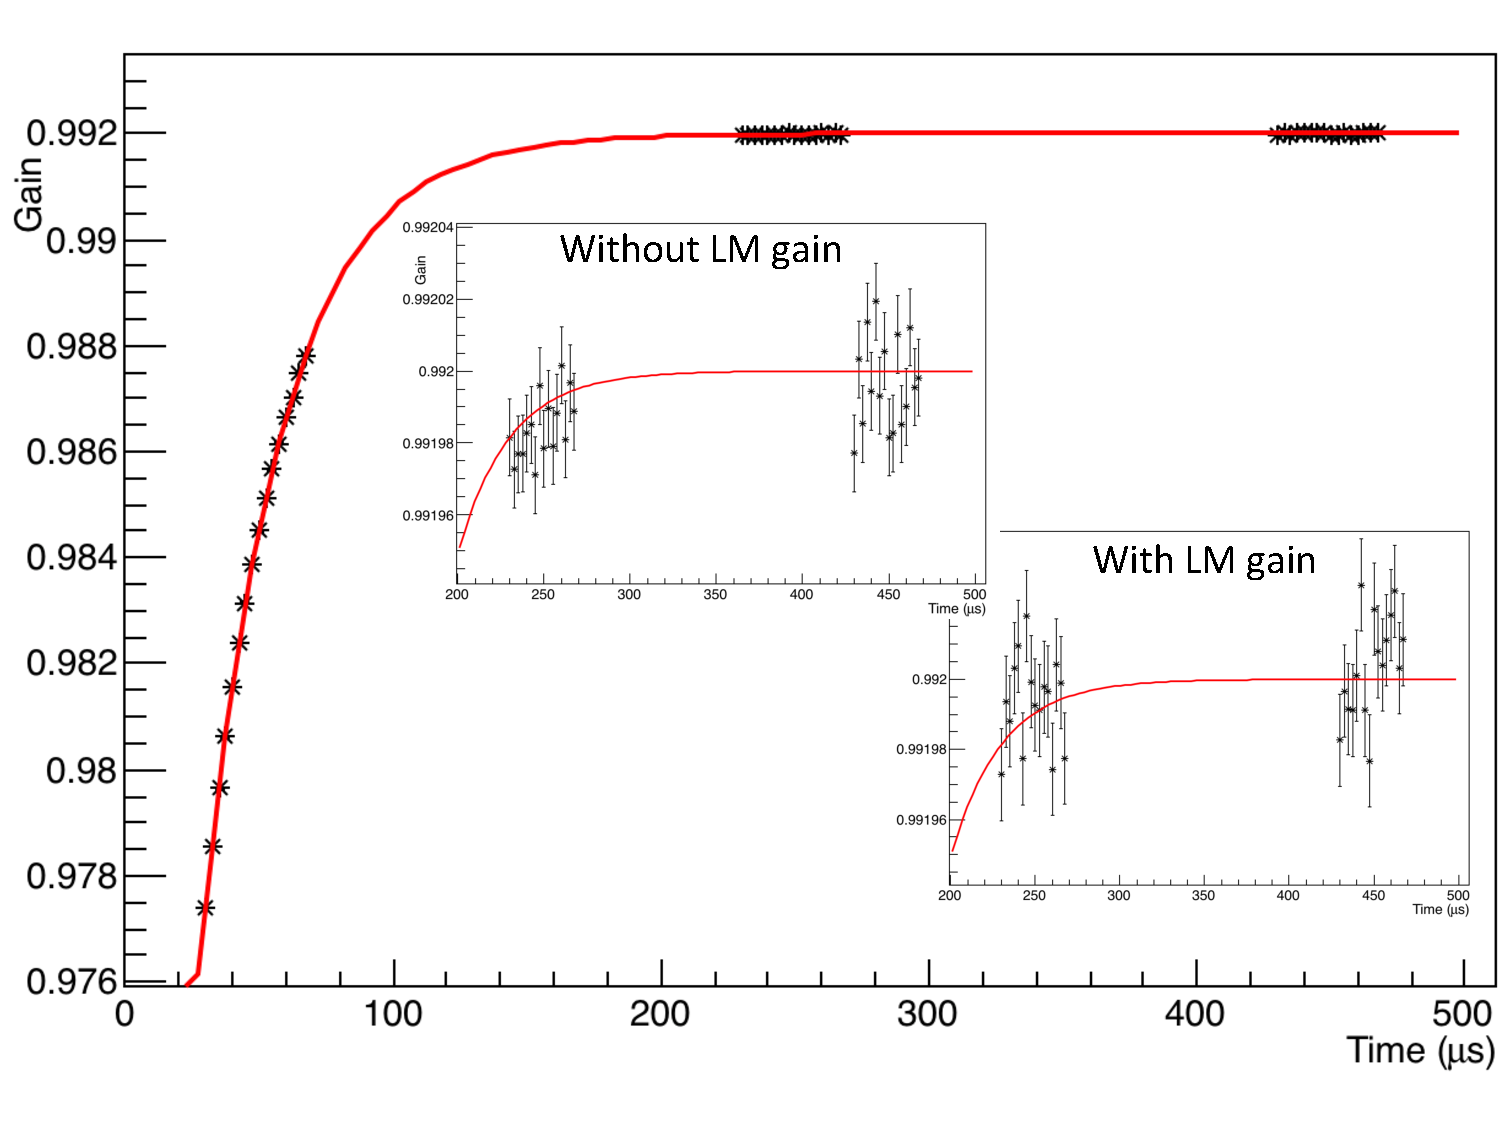
\includegraphics[width=7 cm]{gain_sim.pdf}
\caption{\label{fig7}Left: A fit of the LM amplitude (gain). Right: A simulation - the effect of LMs in the SiPM gain. 
SiPM gain function without any effect of LM (top left) and including a LM gain function (bottom right). }
\end{figure}  
where the subscript i denotes the i$^{th}$ sub run. The effect is shown in the small bottom plot of the 
right panel of figure \ref{fig7}. 
The small top plot in the same panel does not include the effect of the LMs and the gain function is thus simulated using,
\begin{equation}	
  			\begin{aligned}	
    			&\Bigg \langle \frac {(\frac{Q}{S0})_{i}}{\langle {\frac{Q}{S0}}\rangle}_{OOF} \Bigg \rangle
			\end{aligned}
		\end{equation}  

It is evident that there is no noticeable effect of long--term LM fluctuations on the gain function. 
We tried using ten times larger gain drop of A1 with temperature and did not get any effect. 
Thus we do not need to correct for these fluctuations observed by the LM at our desired level of precision. 

\section{Conclusions}
Finally, from this study we conclude the following:
A1 primarily indicates the gain fluctuation of the PMT, as it is directly
 connected to the PMT from the SM using a silica fiber. As expected, all channels show a 
negative correlation with temperature with A1 (PMT gain). 
A2 can have additional effects in fluctuation due to forward and reverse fibers to and 
from the calorimeters respectively. For silica, no visible effects found on A2
 (besides the Gain variation with temperature).
For PMMA there is a significant drop in gain variation with temperature, thus making it 
unsuitable for use. 
The simulation shows that we do not need to correct for these fluctuations 
observed by the LM at our desired level of precision. 
%%%%%%%%%%%%%%%%%%%%%%%%%%%%%%%%%%%%%%%%%% Please edit

\section*{Acknowledgments}
I would like to express my gratitude to Anna Driutti who helped me with the production of this dataset 
and Carlo Ferrari who helped me understand the hardware setup of our laser calibration system. 
Besides, I also appreciate the valuable suggestions given by Graziano Venanzoni, Marco Incagli, Franco Bedeschi 
and several others of our Italian g-2 group. 

%%%%%%%%%%%%%%%%%%%%%%%%%%%%%%%%%%%%%%%%%%
%=====================================
% References, variant A: internal bibliography
%=====================================
\reftitle{References}
\begin{thebibliography}{999}
% Reference 1
\bibitem{anas}
A. Anastasi et al. {\em Nucl. Instrum. Meth. A 842} {\bf 2017} 86.
\bibitem{c2}
G. Pauletta et al. {\em OAHOST, Volume 1, Number 1}, Article Number 5 {\bf 2017}.
\bibitem{c3}
M. Iacovacci et. al.{\em NIMA Proceedings-D-18-00301}  {\bf 2018} - Submitted.
\bibitem{c4}
S. Mastroianni et. al.{\em NIMA Proceedings-D-18-00301} {\bf 2018} - Submitted.
\bibitem{c5}
D. A. Sweigart [Muon g-2 Collaboration], {\em PoS ICHEP} {\bf 2016}, 845 (2016).
\bibitem{TDR}
J. Grange, et al. Fermilab. Muon (g-2) Technical Design Report: -FN0992-E.
% Reference 2
%\bibitem[Author2(year)]{ref-book}
%Author2, L. The title of the cited contribution. In {\em The Book Title}; Editor1, F., Editor2, A., Eds.; 
%Publishing House: City, Country, 2007; pp. 32-58, ISBN.
\end{thebibliography}

\end{document}
